\begin{figure}
    \centering
  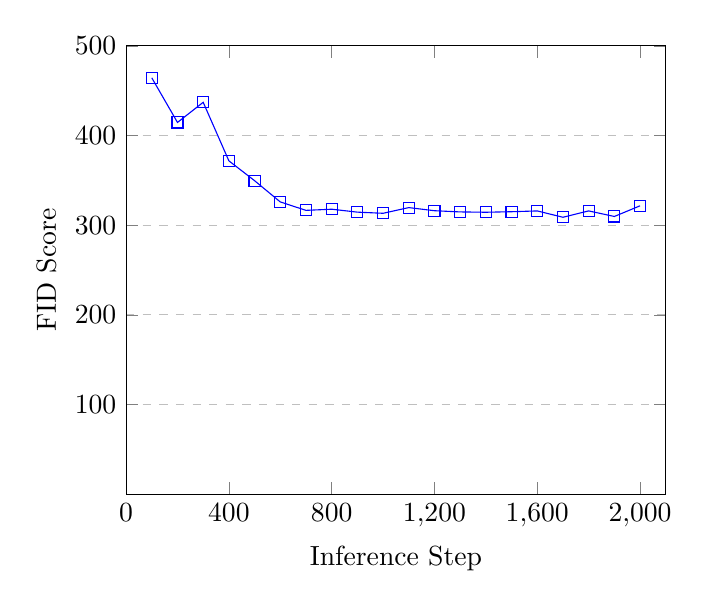
\begin{tikzpicture}
  \begin{axis}[
      xlabel={Inference Step},
      ylabel={FID Score},
      xmin=0, xmax=2100,
      ymin=0, ymax=500,
      xtick={0,400,800,1200,1600,2000},
      ytick={100,200,300,400,500},
      ymajorgrids=true,
      grid style=dashed,
  ]
  
  \addplot[
      color=blue,
      mark=square,
      ]
      coordinates {
        (100,464.27)(200,414.54)(300,436.99)(400,371.72)(500,349.58)(600,325.88)(700,316.48)(800,317.76)(900,314.49)(1000,313.22)(1100,319.56)(1200,316.08)(1300,314.74)(1400,314.38)(1500,314.96)(1600,315.84)(1700,308.78)(1800,315.87)(1900,309.66)(2000,321.56)
      };
      
  \end{axis}
  \end{tikzpicture}
    \caption{For the Smithsonian Butterfly dataset, as the number of noise additions increased, there was a change in the FID score of the images generated by the diffusion model.}
    \label{fig:butterfly_fid}
  \end{figure}